% TODO
% - Sand, Seth, et al. Virgo: blue stars with nothing else

\documentclass[modern]{aastex62}
\usepackage{amsmath}
\graphicspath{{./}{figures/}}

% typography
\setlength{\parindent}{1.\baselineskip}
\newcommand{\acronym}[1]{{\small{#1}}}
\newcommand{\project}[1]{\textsl{#1}}
\newcommand{\package}[1]{\textsl{#1}}
\newcommand{\gaia}{\textsl{Gaia}}
\newcommand{\pans}{\acronym{PS1}}
\newcommand{\decam}{DECam}
\newcommand{\DR}[1]{\acronym{DR#1}}
\newcommand{\todo}[1]{{\color{red} TODO: #1}}
\newcommand{\bs}[1]{\boldsymbol{#1}}

\newcommand{\articlename}{\textsl{Letter}}
\newcommand{\sectionname}{Section}

% Stats / probability
\newcommand{\given}{\,|\,}
\newcommand{\norm}{\mathcal{N}}

% Maths
\newcommand{\dd}{\mathrm{d}}
\newcommand{\transpose}[1]{{#1}^{\mathsf{T}}}
\newcommand{\inverse}[1]{{#1}^{-1}}
\newcommand{\argmin}{\operatornamewithlimits{argmin}}
\newcommand{\mean}[1]{\left< #1 \right>}
\newcommand{\mat}[1]{\mathbf{#1}}

% Units
\newcommand{\msun}{\textrm{M}_\odot}
\newcommand{\kpc}{\textrm{kpc}}
\newcommand{\kms}{\ensuremath{\textrm{km}~\textrm{s}^{-1}}}
\newcommand{\masyr}{\ensuremath{\textrm{mas}~\textrm{yr}^{-1}}}

% Astronomy
\newcommand{\feh}{\ensuremath{[\textrm{Fe} / \textrm{H}]}}
\newcommand{\vlsr}{$V_{\rm LSR}~$}
\newcommand{\vlsre}{$V_{\rm LSR}$}
\newcommand{\hi}{H{\footnotesize I} }
\newcommand{\hie}{H{\footnotesize I}}
\newcommand{\lms}{$L_{\rm MS}~$}
\newcommand{\lmse}{$L_{\rm MS}$}
\newcommand{\bms}{$B_{\rm MS}~$}
\newcommand{\bmse}{$B_{\rm MS}$}

% Shortcuts for this paper
\newcommand{\clustername}{\textsl{Price-Whelan 1}}
\newcommand{\lmcsmc}{LMC--SMC}
\newcommand{\bprp}{\ensuremath{\textrm{BP} - \textrm{RP}}}
\newcommand{\truepm}{\ensuremath{\tilde{\bs{\mu}}}}
\newcommand{\isodist}{\ensuremath{25~\kpc}}
\newcommand{\eep}{\ensuremath{\acronym{\textrm{EEP}}}}

%% Reintroduced the \received and \accepted commands from AASTeX v5.2
% \received{January 1, 2018}
% \revised{January 7, 2018}
% \accepted{\today}

\submitjournal{ApJL}
\shorttitle{Recent star formation in the Magellanic Stream}
\shortauthors{Price-Whelan et al.}

\begin{document}

% \title{A young star cluster in the Galactic halo: \\
% Recent star formation associated with the Leading Arm of the Magellanic stream}
\title{A star formation event in the leading arm of the Magellanic stream triggered by passage through the outer Galactic disk}

\author[0000-0003-0872-7098]{Adrian~M.~Price-Whelan}
\affiliation{Department of Astrophysical Sciences,
             Princeton University, Princeton, NJ 08544, USA}
\email{adrn@astro.princeton.edu}
\correspondingauthor{Adrian M. Price-Whelan}

\author[0000-0002-1793-3689]{David~L.~Nidever}
\affiliation{Department of Physics, Montana State University, P.O. Box 173840, Bozeman, MT 59717, USA}
\affiliation{National Optical Astronomy Observatory, 950 North Cherry Ave, Tucson, AZ 85719, USA}

\author[0000-0003-1680-1884]{Yumi~Choi}
\affiliation{Department of Physics, Montana State University, P.O. Box 173840, Bozeman, MT 59717, USA}
\affiliation{Steward Observatory, University of Arizona, 933 North Cherry Avenue, Tucson AZ, 85721, USA}

\author[0000-0002-8537-5711]{Timothy~Morton} % TODO: check orcID
\affiliation{Department of Astrophysical Sciences,
             Princeton University, Princeton, NJ 08544, USA}

\author[0000-0002-3569-7421]{Edward~F.~Schlafly}
\affiliation{Lawrence Berkeley National Laboratory, One Cyclotron Road, Berkeley, CA 94720, USA}

\author[0000-0003-2808-275X]{Douglas~P.~Finkbeiner}
\affiliation{Institute for Theory and Computation, Harvard-Smithsonian Center for Astrophysics, 60 Garden Street, MS-51, Cambridge, MA 02138, USA}

\author[0000-0003-2644-135X]{Sergey E. Koposov}
\affiliation{McWilliams Center for Cosmology, Department of Physics, Carnegie Mellon University, 5000 Forbes Avenue, Pittsburgh, PA 15213, USA}
\affiliation{Institute of Astronomy, University of Cambridge, Madingley Road, Cambridge CB3 0HA, UK}

\author[0000-0002-0038-9584]{Vasily Belokurov}
\affiliation{Institute of Astronomy, University of Cambridge, Madingley Road, Cambridge CB3 0HA, UK}
\affiliation{Center for Computational Astrophysics, Flatiron Institute, 162 5th Avenue, New York, NY 10010, USA}


\begin{abstract}

We report the discovery of a young, $\sim 150~\textrm{Myr}$, metal-poor, $[\textrm{Fe}/\textrm{H}] \sim -1.2$, stellar association in the halo of the Milky Way, $(R, z) \sim (24, 16)~\textrm{kpc}$. % TODO: check with new dist.
The association --- \clustername\ --- is spatially near the leading arm of the gas stream emanating from the Magellanic cloud system, but is located $\approx 60^\circ$ from the Large Magellanic Cloud (LMC) center, on the other side of the Milky Way disk relative to the LMC.
By assuming that the cluster is co-located with \hi gas in the stream, we directly measure the distance to the Magellanic stream, $d \approx 30~\textrm{kpc}$.
At this location relative to the LMC, the measured distance is inconsistent with predictions from models of the LMC/SMC interaction and infall into the Milky Way that do not account for ram pressure and gas interaction with MW disk.
The estimated age of \clustername\ is consistent with the time of last passage through the Galactic midplane.
We therefore speculate that this star-formation event was triggered by the last disk midplane passage of the Magellanic stream gas, which occurred at a Galactocentric radius $R \approx XX~\kpc$.
However, most details of this idea remain a mystery: the Magellanic Stream is low column density, the Milky Way disk at this large radius has low surface density, and the relative velocity of the gas is large.
Spectroscopic follow-up is needed to confirm its kinematic association with the Magellanic Stream \hi, but either way \todo{this is an interesting thing.}
\end{abstract}

\keywords{Galaxy: halo}


\section{Introduction} \label{sec:intro}

The halo of the Milky Way is characterized by its old ($\gtrsim 10~\textrm{Gyr}$), metal-poor ($\feh \approx -1.5$) stellar population.
This is understood as a signature of the dominant (in stellar mass) progenitor systems that were accreted and disrupted early on in the formation of the Galaxy: massive dwarf galaxies \citep[e.g.,][]{Deason:2015, Fiorentino:2015}.
These systems likely came in with significant gas reservoirs, but were quenched and stripped through collisional processes that heated and dispersed the gas \citep[e.g.,][]{Mayer:2006}, thus preventing immediate star formation in the deposited gas.
The Milky Way, however, continues to accrete satellite galaxies, as is evidenced by the prominent stellar stream from the Sagittarius dwarf galaxy \citep{Ibata:1994, Majewski:2003}, the presence of the Large and Small Magellanic Clouds (LMC, SMC) and about 50 dwarf satellites within the virial radius of the Galaxy.
While Sagittarius was likely stripped of its neutral gas long ago through repeated passage about the Milky Way \citep{Burton:1999, Tepper-Garcia:2018}, the \lmcsmc\ system is associated with $\approx 8\times 10^8~\msun$ of \hi gas \citep{Bruns:2005}, which extends into leading and trailing gas streams that wrap nearly $\approx 200^\circ$ around the sky \citep{Mathewson:1974, Putman:1998, Bruns:2005, Nidever:2010}.

The Magellanic stream (MS) is a large stream of (predominantly) hydrogen gas emanating from the \lmcsmc\ system that contains a significant fraction of the total gas mass associated with the \lmcsmc\ \citep{Bruns:2005}.
The stream was discovered in early surveys of 21 cm emission and has since been studied in great detail by large-area radio sky surveys, and in H$\alpha$ emission \citep{Weiner:1996, Barger:2017}.
With increased resolution, surveys have found small-scale structure and gas fragmentation \citep[e.g.,][]{Nidever:2008, For:2014} and a large-scale bifurcation, with %semi-distinct ``strands'' that lead back to the LMC and broader system, respectively \citep[e.g.,][]{Morras:1983, Putman:2003}.
kinematically \citep{Nidever:2008} and chemically \citep{Fox:2013} distinct ``strands'' that lead back to the LMC and the SMC, respectively.
As surveys push deeper to lower column densities, extensions of the stream have been found both in the trailing region \citep{Nidever:2010}, but also in the leading arm, which has been found to connect to regions of low-column-density gas ($N\sim 10^{18}$--$10^{19}~\textrm{cm}^{-2}$) on the other side of the Galactic disk \citep{Putman:1998, Nidever:2008}.
The leading arm (LA) has been decomposed into three or four distinct ``features'' named LA1--4 \citep{Bruns:2005, Nidever:2008, Venzmer:2012} with total HI mass $\sim 4 \times10^7~\msun$ \citep{Venzmer:2012}.

The origin and formation of the LA features in the MS is still uncertain.
Initial studies of the LA argued that the features closest to the \lmcsmc\ can be traced back to the SMC, thus implying that the gas in the LA was stripped from the SMC \citep{Putman:1998}.
In later work, it has instead been argued that outer features of the LMC appear to lead directly into the LA-1 feature \citep{Nidever:2008}, implying an LMC origin for the leading arm.
Recent chemical abundance measurements along several sightlines passing through the LA again suggested the SMC origin \citep{Fox:2018, Richter:2018}.
Recent hydrodynamical simulations of the MCs on the first infall to the Milky Way, however, showed that the repeated encounters between the MCs strip gas not only from the SMC, but also from the LMC, and this tidally stripped gas creates filamentary gas structures both in the LA and the Magellanic Stream \citep{Pardy:2018}.
Whatever the origin of the gas, it is clear that tidal stripping by the Milky Way is required to form the leading arm \citep{Nidever:2008, Besla:2012}.
However, the LA features deviate from the predicted orbit of the \lmcsmc, implying that ram pressure or interactions with gas in the outer Milky Way disk may have removed orbital energy from the LA gas \citep[e.g.,][]{Bekki:2008}.

Streams formed from tidally stripped material --- such as the Sagittarius or Palomar 5 \citep{Odenkirchen:2001} stellar streams, or gas streams such as the MS --- encode information about the orbital history and future trajectory of their progenitor system \citep[e.g.,][]{Johnston:1999}.
For this reason, streams of debris are of interest for constraining the dark matter distribution around the Galaxy, as well as for providing a fossil record of the Milky Way's accretion history \citep{Johnston:1998, Bullock:2005}.
Several groups have attempted to use the MS to constrain both the infall history of the \lmcsmc\ and the dark matter halo of the Milky Way (see recent review by \citealt{DOnghia:2016}).
Early models for the formation of the MS invoke ram pressure and tidal stripping to explain the sky distribution and extent of the MS, and typically require that the \lmcsmc\ system complete several orbits around the Galaxy in order to strip enough material \citep[e.g.,][]{Murai:1980, Gardiner:1994, Mastropietro:2005}.
However, later measurements of the proper motion of the LMC (\citealt{Kallivayalil:2006}, later confirmed by \gaia\ \citealt{van-der-Marel:2016}) and improved models for the infall dynamics \citep{Besla:2007} suggest instead that the \lmcsmc\ system could be on its first passage through the Galaxy \citep{Besla:2010, Besla:2012}.
In addition, the orbit of the LMC implied by the new proper motion measurement appears to be offset by $\approx 10^\circ$ from the trailing MS \citep{Besla:2010}.
Put together, these recent revelations have led to new models for the formation of the MS that largely rely on past interactions between the LMC and SMC to preprocess the gas distribution before infall and eventual stripping by the tidal field of the Milky Way \citep{Besla:2012, Diaz:2012}.

One critical difficulty in using the MS to constrain models of the \lmcsmc\ interaction and infall is the lack of distance information along the stream.
No significant over-density of stars have been found associated with the trailing portion of the MS \citep{Guhathakurta:1998}, thus leaving distance and tangential velocity information largely unknown.
Recently, a small number of young OB stars have been found in the vicinity of the leading arm gas, with radial velocities consistent with having formed from the leading MS \citep{Casetti-Dinescu:2014, Zhang:2017}.
However, given their sparsity and concentration near the Galactic plane, it is difficult to unambiguously associate them with the MS: these could instead be runaway OB stars from the Milky Way disk.

In this \articlename, we report the discovery of a clustered association of young stars at the far edge of the LA-2 feature ($L_{\textrm{MS}} \sim 65^\circ$) that is unambiguously located far into the Galactic halo ($d_\odot \sim 30~\textrm{kpc}$) and therefore likely formed from gas in the leading arm of the Magellanic stream as it crossed the Galactic disk.
This provides a clear distance measurement to the leading arm of the MS to be compared with models of \lmcsmc\ interaction and infall into the Milky Way, and also provides an opportunity to study recent star formation in a regime unlike that of the Milky Way. \todo{or any other?}

In \sectionname~\ref{sec:data}, we present the initial discovery with \gaia\ \DR{2} and follow-up observations with DECam to obtain deeper photometry of the region around the association.
In \sectionname~\ref{sec:results}, we derive estimates for the total stellar mass of, age of, and distance to the association, and present a plausible formation scenario.
In \sectionname~\ref{sec:discussion}, we discuss implications for future searches for stars associated with the MS, and discrepancies with existing models of the LA.
We conclude in \sectionname~\ref{sec:conclusion}.

\section{Data} \label{sec:data}

\subsection{Cluster discovery with \gaia}
\label{sec:discovery}

We use astrometric data from the \gaia\ mission (\citealt{Prusti:2016}), data release 2 (\DR{2}; \citealt{Gaia-Collaboration:2018, Lindegren:2018}) to search for distant, comoving multiplets of blue stars.
Our original intent was to search for small, distant, comoving groups of blue horizontal branch stars to identify new candidate satellites of the Milky Way.
We therefore initially select all stars from \gaia\ with parallax $\varpi < 1$, color $-0.5 < (\bprp) < 0$, $G$-band magnitude $G < 20$, and Galactic latitude $|b| > 20^\circ$ (see Appendix~\ref{sec:queries} for database query).
We further exclude stars within a $15^\circ$ radius from the LMC, and a $8^\circ$ radius from the SMC --- 27,895 stars remain after these cuts.
We then cross-match this catalog to itself with both sky positions and proper motions: we search for pairs of stars that have separations $s < 0.5^\circ$ and proper motion differences $|\Delta \mu| < 0.5~\masyr$.
We then combine mutually-connected comoving pairs into small groups of stars that are colocated on the sky and comoving in proper motions, and remove groups that have $<4$ members.
We cross-match the mean sky positions of the groups to locations of local group galaxies \todo{citation} \citep{Mcconaghie} and Milky Way globular clusters \todo{citation} \citep{Harris} and filter out all groups that lie within 1 degree of these known objects.
After these filters, just one group of blue, comoving stars remains at $(\textrm{RA}, \textrm{Dec}) \sim (179, -29)^\circ$.

We then query all objects from the \gaia\ \DR{2} catalog within a rectangle centered on the nominal position of this group, with a width of $12^\circ$ and a height of $12^\circ$ in the equatorial (ICRS) coordinate system (see Appendix~\ref{sec:queries} for the database query).
We cross-match the resulting catalog with \acronym{GALEX} \citep{Martin:2005} using a positional cross-match requiring source separation $<2~\textrm{arcsec}$, and with \pans\ \citep{Chambers:2016} using the cross-match provided by the \gaia\ science archive.
\figurename~\ref{fig:cmds} shows the \gaia\ color-magnitude diagram (left) and the \acronym{GALEX} NUV minus \pans\ $g$-band versus \gaia\ \bprp\ color-color diagram (right) from the cross-matched photometry.
All magnitudes are corrected for dust extinction using the SFD \citep{Schlegel:1998, Sclafly:2011} dust map.
The green polygon in the left panel of \figurename~\ref{fig:cmds} highlights the over-density of blue stars that were identified as comoving from the proper motion search described above: surprisingly, this appears to be a young, distant main sequence, rather than an old population of horizontal branch stars.
The lines in the right panel of \figurename~\ref{fig:cmds} show isochrones from the \acronym{MIST} \citep[blue;][]{Choi:2016} and \acronym{PARSEC} \citep[red;][]{Bressan:2012, Marigo:2017} isochrone libraries for a 50 Myr stellar population with metallicity $\feh = -0.5$ (dashed) or $\feh = -1.5$ (solid). \todo{Remake this plot with just FeH=-1.}

% Notebook: Figure-CMDs
\begin{figure}
\centering
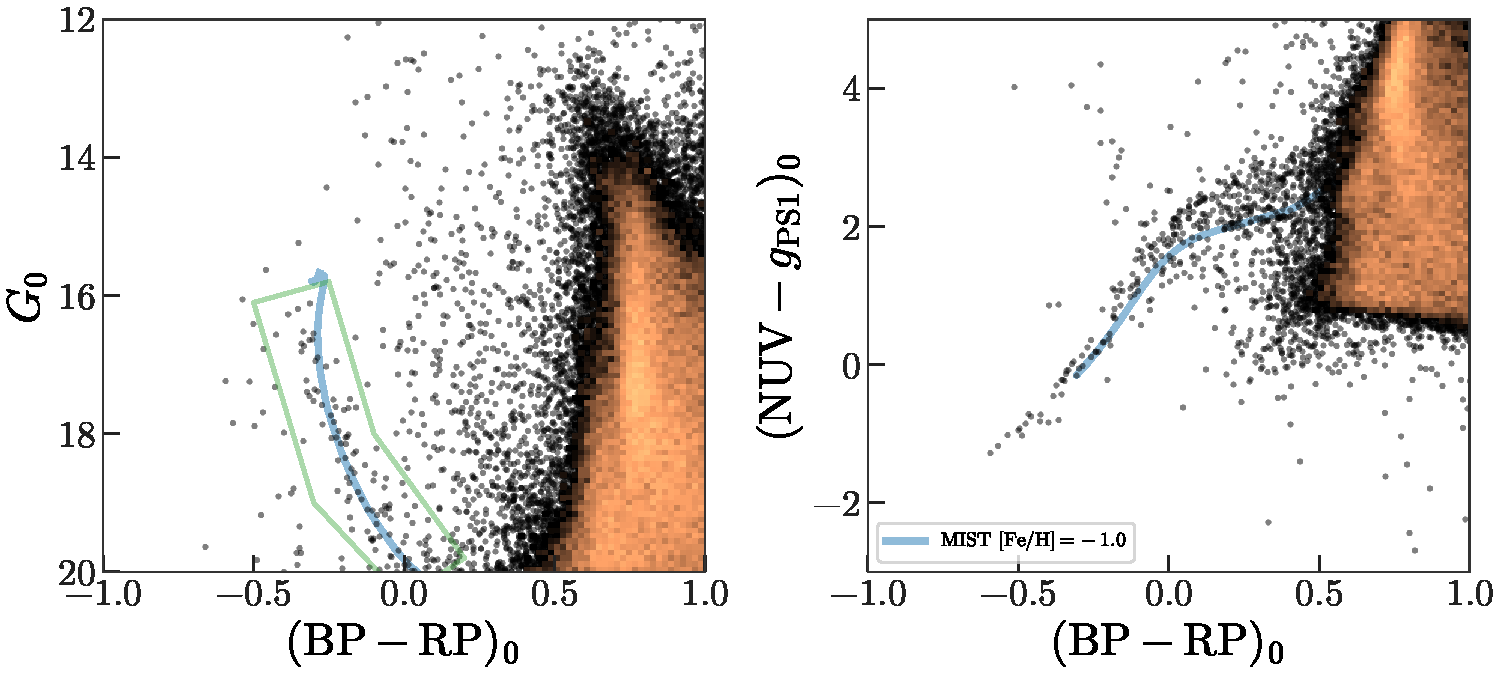
\includegraphics[width=\textwidth]{figures/gaia-galex-cmd.pdf}
\caption{Color-magnitude and color-color diagrams with \gaia\ ($G$, BP, RP), \acronym{GALEX} (NUV), and \pans\ ($g$) magnitudes.
Shaded pixels (orange) show regions of high density and points (black markers) are plotted when there are fewer than 8 stars per pixel.
Green polygon in left panel highlights the over-density of blue, comoving stars identified by the search described in \sectionname~\ref{sec:discovery}.
Red and blue lines in right panel show the zero-age main sequence of a $50~\textrm{Myr}$ stellar population with the metallicity indicated from the \acronym{MIST} \citep{TODO} and \acronym{PARSEC} \citep{TODO} isochrone libraries.
}
\label{fig:cmds}
\end{figure}


\subsection{Follow-up with \decam}
\label{sec:decam}

\todo{Nidever}

% Figure \ref{fig_skypm} shows the spatial and proper motion distribution in the region of interest with the objects in
% a small proper motion selection shown as black and red dots.  The color magnitude diagram (CMD) of the same objects
% is shown in Figure \ref{fig_cmd} and clearly reveals a sequence of objects that follow the shape of a young main-sequence.
% The PS1 photometry of the same region is shown in Figure \ref{fig_isochrone} and as well as young, metal-poor isochrones at fa distance of 25 kpc.  Finally, Figure \ref{fig_gass} shows a position-velocity diagram at the position of the cluster of the \citep[GASS;][]{McClure-Griffiths:2009} \hi data that has been Gaussian decomposed using the technique in \citet{Nidever:2008}.
% The component of the LA II can be seen on the left-hand side of the figure and a similar \hie stream can be seen near the
% position of the cluster.
% Yumi:
% Need a sentence or two for dust extinction correction somewhere in the above two paragraphs?


\section{Methods} \label{sec:methods}

In the subsections below, we perform two independent analyses of the data available for \clustername.
In \sectionname~\ref{sec:pmclean}, we use astrometric data from \gaia\ \DR{2} to identify members probabilistically, then demonstrate that the high-probability kinematic members appear as a clear young main sequence in the \gaia\ CMD.
In \sectionname~\ref{sec:popmodel}, we use photometric data from \decam\ to again identify members probabilistically, and simultaneously infer the cluster parameters (age, metallicity, distance, etc.).
We perform these analyses separately because \gaia\ \DR{2} only includes the most massive members of the cluster, but the addition of lower main sequence members apparent in the \decam\ photometry provide a much better constraint on the cluster parameters.

\subsection{Determining kinematic membership}
\label{sec:pmclean}

We select probable members of \clustername\ by constructing a probabilistic model of the cluster and background population using astrometric data from \gaia.
We start by selecting all stars with $\bprp_0 < 0.35$ to remove low-mass and old main sequence star contamination in the region.
\figurename~\ref{fig:pm-members}, left (grey points), shows the sky positions of stars that pass this blue cut in the region around the young cluster.
The larger solid-line (green) circle indicates the region we define as the cluster area, and the two smaller dashed-line (blue) circles indicate control fields that are combined and used for modeling the background distribution of proper motions.
The control fields are designed to, together, have the same total area as the cluster field.
The top-left panel of the middle panels shows the proper motion distribution in the control fields, and top-right panel in the middle shows the proper motion distribution of the cluster field.
The distinct over-density of stars near $(\mu_\alpha, \mu_\delta) \approx (-0.5, 0.5)~\masyr$\footnote{Throughout this article, we use $\mu_\alpha$ to refer to the proper motion value provided by \gaia, which includes the $\cos\delta$ term.} is the identified comoving association of blue stars.

To model membership of the cluster based on the observed proper motions, $\bs{\mu} = (\mu_\alpha, \mu_\delta)$, we first construct a model for the error-deconvolved proper motion distribution in the control fields using ``extreme deconvolution'' \citep[XD;][]{TODO} with two Gaussian components.
The bottom-left panel of the middle panels of \figurename~\ref{fig:pm-members} shows the $2\sigma$ contours of the two inferred Gaussian components (blue) from running XD, which takes into account the full error distributions for each proper motion measurement (i.e. including covariances), $\mat{C}_\mu$, provided by \gaia\ \DR{2}.
After running XD, we fix the parameters of the background model and model the cluster field proper motion distribution using a two-component mixture model with a single, isotropic Gaussian component for the error-deconvolved cluster distribution with mean $\bs{m}$ and isotropic variance $s^2$, and the XD-inferred model for the control field, $p_{\textrm{XD}}$, for the background component.
In detail, taking $f$ to be the fraction of blue stars in this region belonging to the young cluster, and \truepm\ to be the true proper motion for a single star,
\begin{align}
    p(\bs{\mu} \given \truepm, \mat{C}_\mu) &=
        \norm(\bs{\mu} \given \truepm, \mat{C}_\mu)\\
    p(\truepm \given f, \bs{m}, s) &=
        f \, p_{\textrm{cl}}(\truepm \given \bs{m}, s)
        + (1-f) \, p_{\textrm{XD}}(\truepm)\\
    p_{\textrm{cl}}(\truepm \given \bs{m}, s) &=
        \norm(\truepm \given \bs{m}, s^2 \, \mathbb{I})
\end{align}
where $\norm(\bs{x} \given \bs{m}, \mat{C})$ represents the multidimensional normal distribution with mean $\bs{m}$ and covariance matrix $\mat{C}$, and $\mathbb{I}$ is the identity matrix.
Because all distributions are Gaussian, the per-star parameters (the true proper motions, \truepm) can be analytically marginalized out so that the per-star likelihood can be expressed as $p(\bs{\mu} \given f, \bs{m}, s, \mat{C}_\mu)$.
We assume that the measurements for each star, $n$, are independent so that the full likelihood of all $N$ stars given the parameters $(f, \bs{m}, s)$ is
\begin{align}
    p(\{\bs{\mu}_n\}_N \given \given f, \bs{m}, s, \{\mat{C}_{\mu, n}\}_N) &=
        \prod_n^N p(\bs{\mu}_n \given f, \bs{m}, s, \mat{C}_{\mu, n}) \quad .
        \label{eq:likelihood}
\end{align}

We use an ensemble Markov chain Monte Carlo (MCMC) sampler \citep[\texttt{emcee};][]{Goodman:XX, Foreman-Mackey:2013} to generate posterior samples over the parameters $(f, \bs{m}, s)$ using the likelihood defined above (Equation~\ref{eq:likelihood}), and assuming the following prior probability distributions: uniform over the domain $(-5, 5)~\masyr$ for each component of $\bs{m}$, uniform in $f$, and uniform in log-$s$ over the domain $-6 < \ln s < 4$ (with $s$ in units of \masyr).
We run the sampler with 32 walkers for 256 steps as burn-in, then reset the sampler and run for an additional 512 steps.
We then thin the resulting chains by taking every 16th sample, leaving a total of 1024 samples; We use these samples to estimate the median posterior parameter values and uncertainties, and to compute, for each star, posterior probabilities of belonging to the cluster mixture component.
For the young cluster, we find $\bs{m} = (-0.56,  0.47) \pm (0.04, 0.02)~\masyr$, $\ln s = -3.8 \pm 0.9$, and $f = 0.14 \pm 0.02$.
The bottom-left panel of the middle panels of \figurename~\ref{fig:pm-members} shows, in black (small black ellipse), the inferred median proper motion and proper-motion dispersion of the young cluster.
The proper-motion dispersion is consistent with zero, but is unmeasured; 95\% of the posterior samples have $s < 0.09~\masyr$.

The bottom-right panel of the middle panels of \figurename~\ref{fig:pm-members} shows all stars in the cluster field, but each marker is colored by the probability of (kinematically) belonging to the young cluster.
The right (large) panel of \figurename~\ref{fig:pm-members} shows the sky positions of all stars with $\textrm{probability} > 0.5$ of belonging to the cluster: These comoving, blue stars show a clear spatial over-density in this region.

To further validate the existence of this cluster, we visualize the \gaia\ color-magnitude diagrams of the high-probability members in both the control and cluster fields (see leftmost panel of \figurename~\ref{fig:pm-members}).
\figurename~\ref{fig:pm-members-cmd} shows the CMDs for all stars in this sky region (grey background) in both panels, and stars with $\text{probability} > 0.5$ of belonging to the young cluster (black markers) in the control field (left, 5 stars) and cluster field (right, 65 stars).
The colored lines show $\feh = -1$ isochrones with ages indicated at a distance of 30~\kpc.
In the next section, we model the distribution of stars in the \decam\ color-magnitude diagram to determine the characteristics of the stellar population.

% Notebook: Proper-motion-membership
\begin{figure}
\centering
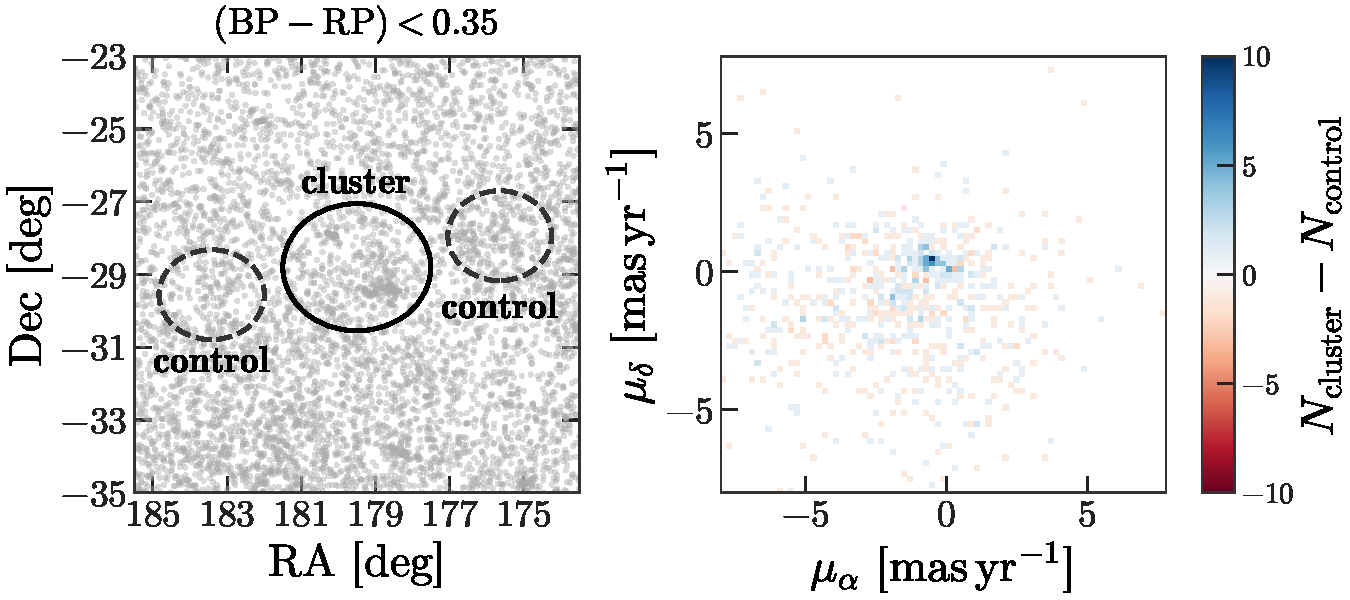
\includegraphics[width=\textwidth]{figures/pm-model.pdf}
\caption{\todo{APW}
Add proper motion vector?}
\label{fig:pm-members}
\end{figure}

% Notebook: Proper-motion-membership
\begin{figure}
\centering
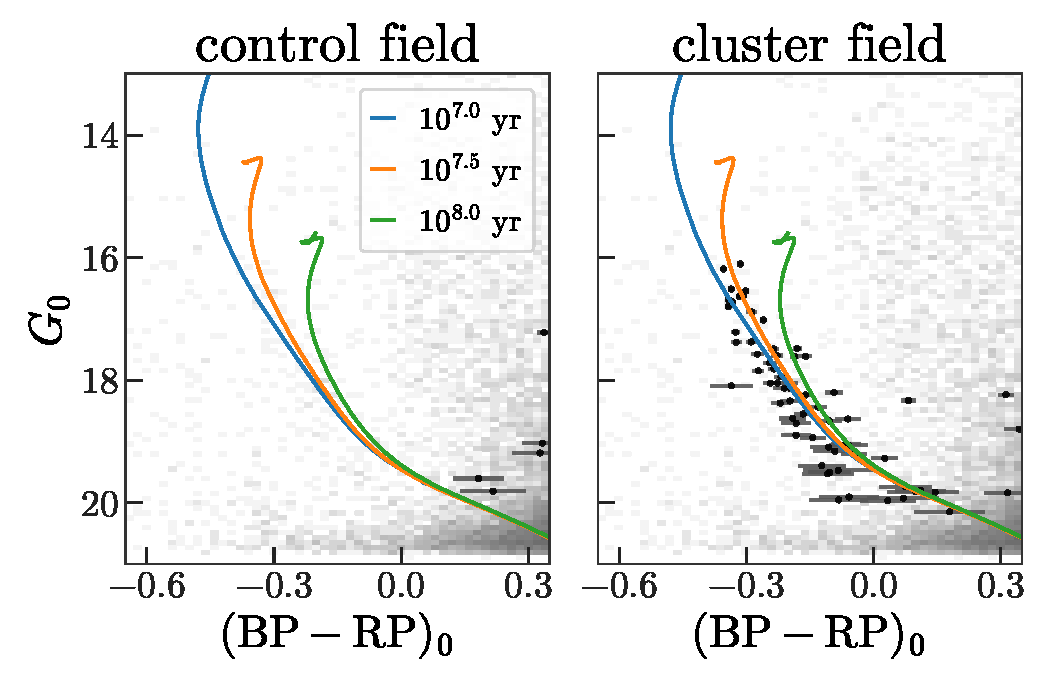
\includegraphics[width=0.6\textwidth]{figures/pm-members-cmd.pdf}
\caption{\gaia\ color-magnitude diagrams for stars in the sky region around \clustername: grey background in both panels shows the distribution for all stars, and black points show stars with $\textrm{probability} > 0.5$ of (kinematically) belonging to \clustername.
Left panel is for stars in the control fields, right panel is for stars in the cluster field.
Colored lines show $\feh = -1$ isochrones from the \acronym{MIST} \citep{TODO} isochrone library for the ages indicated at a distance of \isodist.}
\label{fig:pm-members-cmd}
\end{figure}


\subsection{Stellar population modeling}
\label{sec:popmodel}

The deeper photometry from \decam\ provides a clear view of the stellar population of \clustername\ down to stellar masses $M \sim 0.9~\msun$:
\figurename~\ref{fig:decam-cmd} shows the \decam\ $g$ and $i$ band color-magnitude diagrams for control fields (left) and cluster fields (right) selected from the \decam\ footprint, once again showing the young main sequence (single stellar population in right panel).
We use the $g$- and $i$-band photometry for individual stars in a sub-section of the cluster field CMD (red dashed outlined region in \figurename~\ref{fig:decam-cmd}) to infer the stellar population parameters of \clustername.
To summarize our methodology, we generate posterior samplings over the stellar parameters of each individual source under an interim prior (over age, stellar mass, distance, etc.), then use these individual samplings to construct a Bayesian hierarchical model for a two-component mixture of a single stellar population and a background population.
The results of this modeling are presented in \sectionname~\ref{sec:popchars}.

In detail, we start by using the \texttt{isochrones} package \citep{Morton:XXXX} to generate posterior samplings over stellar parameters for each individual source given its photometry and an interim prior.
We use the \acronym{MIST} \citep{Choi:2016} isochrone library, and \texttt{isochrones} automatically performs interpolation between the provided grid of stellar isochrones to evaluate predicted stellar parameters at a given location in the CMD.
The stellar parameters for each source are its ``equal evolutionary point'' number $\eep$ (see \acronym{MIST} documentation; \citealt{WHO}), age $\tau$, metallicity $\feh$, extinction $A_V$, and distance $D$, which can be uniquely mapped to a point in the observed CMD;
The likelihood of a given set of these parameters, $\boldsymbol{\theta} = (\eep, \tau, \feh, A_V, D)$, is then computed from the photometry and (assumed Gaussian) photometric uncertainties given the predicted photometry.

To generate posterior samples, we must also specify prior probability distributions over the parameters $\boldsymbol{\theta}$.
The priors for each parameter are summarized in \tablename~\ref{tbl:priors}.
The bounds on $\eep$ limit the isochrone to evolutionary phases between the zero-age main sequence to the terminal-age main sequence.
The prior and bounds on $A_V$ are set to prefer small and reasonable values of extinction for this moderately high Galactic latitude region.
The prior on distance assumes a uniform space density of stars.

As expected, we find that the photometry for individual sources in the lower main sequence are very poorly constrained in all parameters, and the prior tends to pull the posterior samplings to prefer closer, older stellar parameters.
This is a weakness of our methodology for performing the hierarchical inference: each source is considered independently, even though there is clear structure in the CMD (i.e. \figurename~\ref{fig:decam-cmd}).
A more correct way to do this would be to infer the stellar parameters of \emph{all} stars, the cluster hyperparameters, and the background simultaneously.
However, for the 417 stars we are using (in the red box in \figurename~\ref{fig:decam-cmd}), this model would have $\sim$2,000 free parameters, if left unmarginalized.
We are developing tools to perform star cluster parameter inference in this way (Morton et al., in prep.), but here we adopt a simple hack to allow us to instead perform individual posterior samplings and then combine into a hierarchical inference.

The brightest stars in the cluster have very precise \decam\ photometry, and have precise astrometry from \gaia, and therefore have membership probabilities from the previous section (\sectionname~\ref{sec:pmclean}).
Given their location in the CMD, these stars must be young, and so also have much better constrained stellar parameters.
We therefore use the brightest, high-probability \emph{kinematic} member --- XXX --- as an ``anchor'' star:
We model every other source (i.e. excluding XXX) in the \decam\ selection region by fitting the photometry of it and the anchor star simultaneously, assuming they have the same age, metallicity, distance, and extinction but different \eep\ values.
Motivated by the possible signature of an (unresolved) binary sequence in the \decam\ CMD, we add one further piece of complexity to the model by allowing the photometry of each non-anchor source to be fit as an unresolved binary star system.
This adds an additional parameter, the unresolved binary mass ratio $q$, to the list of inferred stellar parameters for each source.
The details of this model are handled by the \texttt{isochrones} package.

\begin{table}[ht]
\begin{center}
    \begin{tabular}{ c | c | c }
        \toprule
        Parameter & Prior & Bounds \\
        \toprule
        $\eep$ & uniform & $(202, 355)$ \\
        $\tau$ & uniform & $(10~\textrm{Myr}, 15~\textrm{Gyr})$ \\
        $\feh$ & uniform & $(-2, 0.5)$ \\
        $A_V$ & $\propto A_V^{-1}$ & $(0.001, 1)~\textrm{mag}$ \\
        $D$ & $\propto D^{2}$ & $(1, 100)~\kpc$ \\
        \toprule
    \end{tabular}
\caption{Prior probability distributions for each of the stellar parameters defined in \sectionname~\ref{sec:popmodel}.
\label{tbl:priors}}
\end{center}
\end{table}

In the end, we generate posterior samplings over the parameters $(\boldsymbol{\theta}, q)$ for each of the 417 sources in the selected region of the \decam\ CMD using \texttt{PyMultinest} \citep{TODO}, and store the value of the prior evaluated at the location of each sample.
We then use these samples and interim prior values to construct our hierarchical model.
In the hierarchical model, we assume that the stellar parameters of each primary star in the CMD region are either drawn from the cluster, or a background (stellar halo) population.
For the cluster, we assume the values are drawn from delta functions in age, metallicity, distance, and extinction, with the centroids of the delta functions $\boldsymbol{\alpha} = (\mu_\tau, \mu_{\feh}, \mu_D, \mu_{A_V})$ as hyperparameters of the hierarchical inference. \todo{Double check that we let all 4 of these free}
For the background model, we assume the same priors as specified in \tablename~\ref{tbl:priors}.
The one other parameter of this hierarchical model is the global fraction of sources that are likely cluster members, $f$.
The full XXX of this model for all $K=417$ source ... \todo{write this down}
\begin{align}
    p(\boldsymbol{\theta}_K, q_K, \boldsymbol{\alpha}, f \given \{g, i\}_K )
        &\propto
        \prod_k^K p(g_k, i_k \given \boldsymbol{\theta}_k, q_k) \,
            p(\boldsymbol{\theta}_k, q_k \given \boldsymbol{\alpha}, f) \,
            p(\boldsymbol{\alpha}) \, p(f)
\end{align}
(see \citealt{Hogg:2008, Foreman-Mackey:2013, Price-Whelan:2018} for other examples of this trick). \todo{double check references and add}
\todo{Make a PGM for this model?}

\todo{OK, so now finally we generate samples in alpha, f using emcee, and now we have inferred the cluster parameters - boo ya}

% Notebook: Figure-DECam-CMD
\begin{figure}
\centering
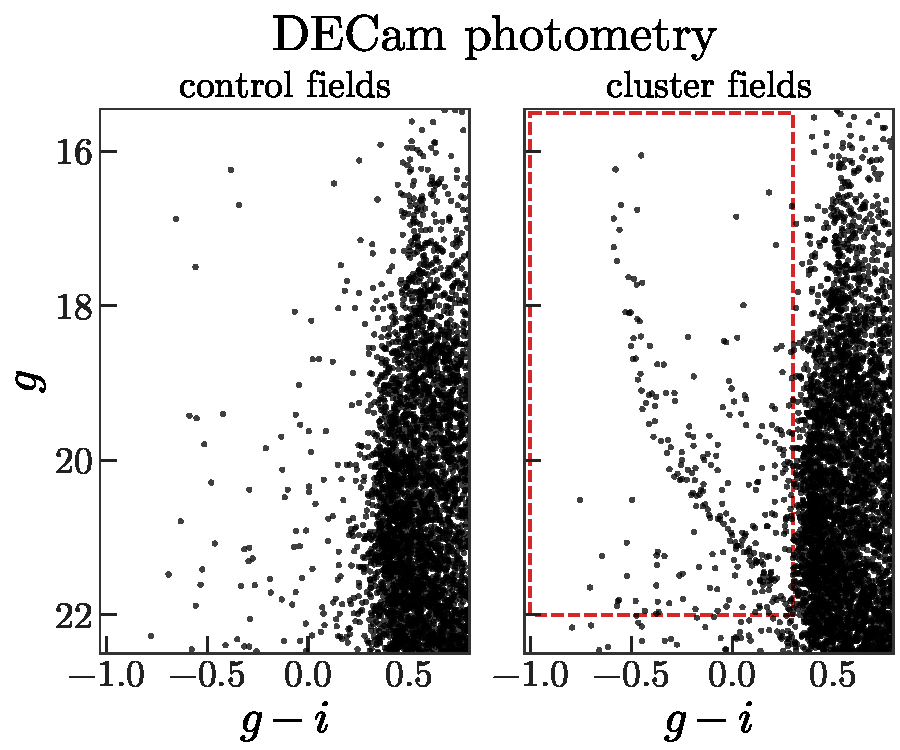
\includegraphics[width=0.6\textwidth]{figures/DECam-cmd.pdf}
\caption{TODO}
\label{fig:decam-cmd}
\end{figure}


\section{Results} \label{sec:results}

\subsection{The stellar population of \clustername}
\label{sec:popchars}

\todo{APW}

% TODO:
% - Stellar mass estimate

\subsection{Relation to \hi gas}
\label{sec:higas}

\todo{Nidever}

We have used the new Gaia data to detect a young, metal-poor cluster in the halo of the Milky Way at a distance of 25 kpc and a MW z-height of 12 kpc.  The detection of such a young cluster so far from the star-forming disks of any nearby
galaxy is highly unusual.  However, the proximity of the new cluster to the Leading Arm of the Magellanic Stream suggests
that the cluster originated from this metal-poor gas \citep{Fox:2018}.  Previously studies have detected young stars in the Leading Arm and gas in the periphery of the Magellanic Clouds \citep{Casetti-Dinescu:2014, MoniBidin:2017}, however, this is the first time that an entire star cluster has been detected so far from the Clouds.

% We evaluate the hypothesis that the cluster formed in the Leading Arm.  The mean proper motion values in the Magellanic Stream coordinate system \citep{Nidever:2008} are ($\mu_{\rm MSL}$,$\mu_{\rm MSB}$)=($+$1.X,0.X) mas yr$^{-1}$ which is very similar to the mean values of the LMC and SMC with ($+$1.X,0.X) mas yr$^{-1}$ and ($+$1.X,0.X) mas yr$^{-1}$, respectively.  The simulations of \citet{Besla:2012} also predict proper motions at this position of approximately ($+$1.X,0.X) mas yr$^{-1}$.  The Magellanic Stream simulations give distances of the Leading Arm at this position of $\sim$50 kpc, however, many of these do not include the effects of ram pressure from the hot MW halo which could cause the gas to drop in its orbit to smaller Galactocentric distances (NEED TO DOUBLE-CHECK THIS).  In addition Figure \ref{fig_gass} shows that there is Leading Arm \hi~gas at the position of the position of the cluster with a velocity of \vlsr=70 \kmse.


\begin{figure}
\centering
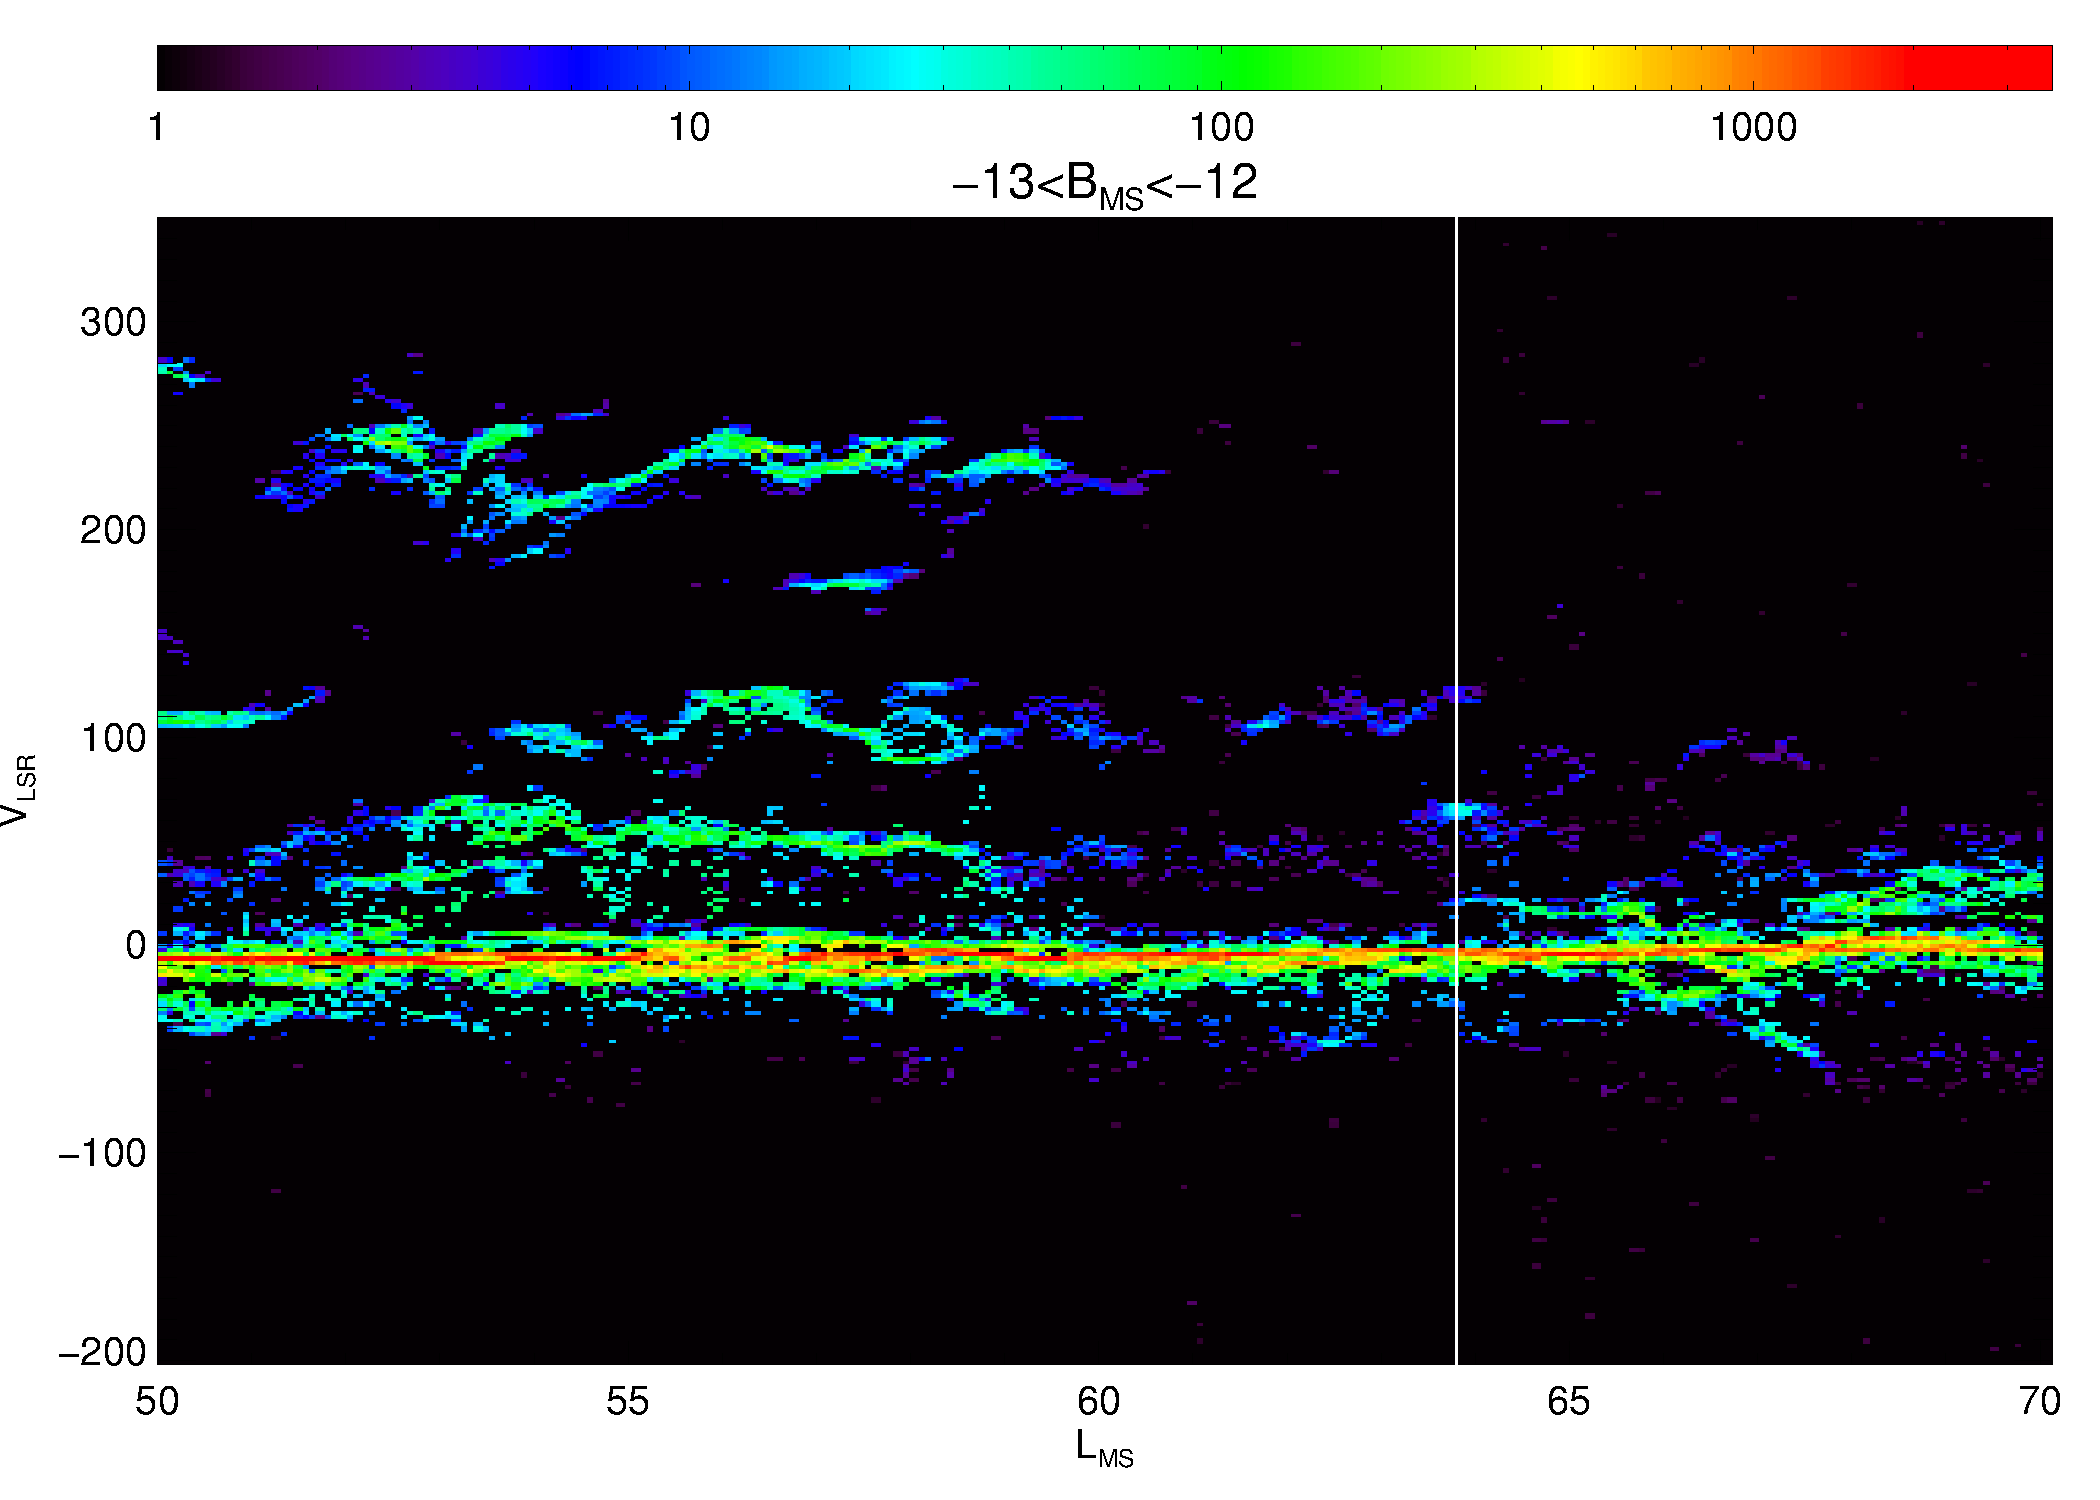
\includegraphics[width=8cm]{gass_vlsrmlon.pdf}
\caption{GASS position-velocity diagram.}
\label{fig_gass}
\end{figure}

\begin{figure}
\centering
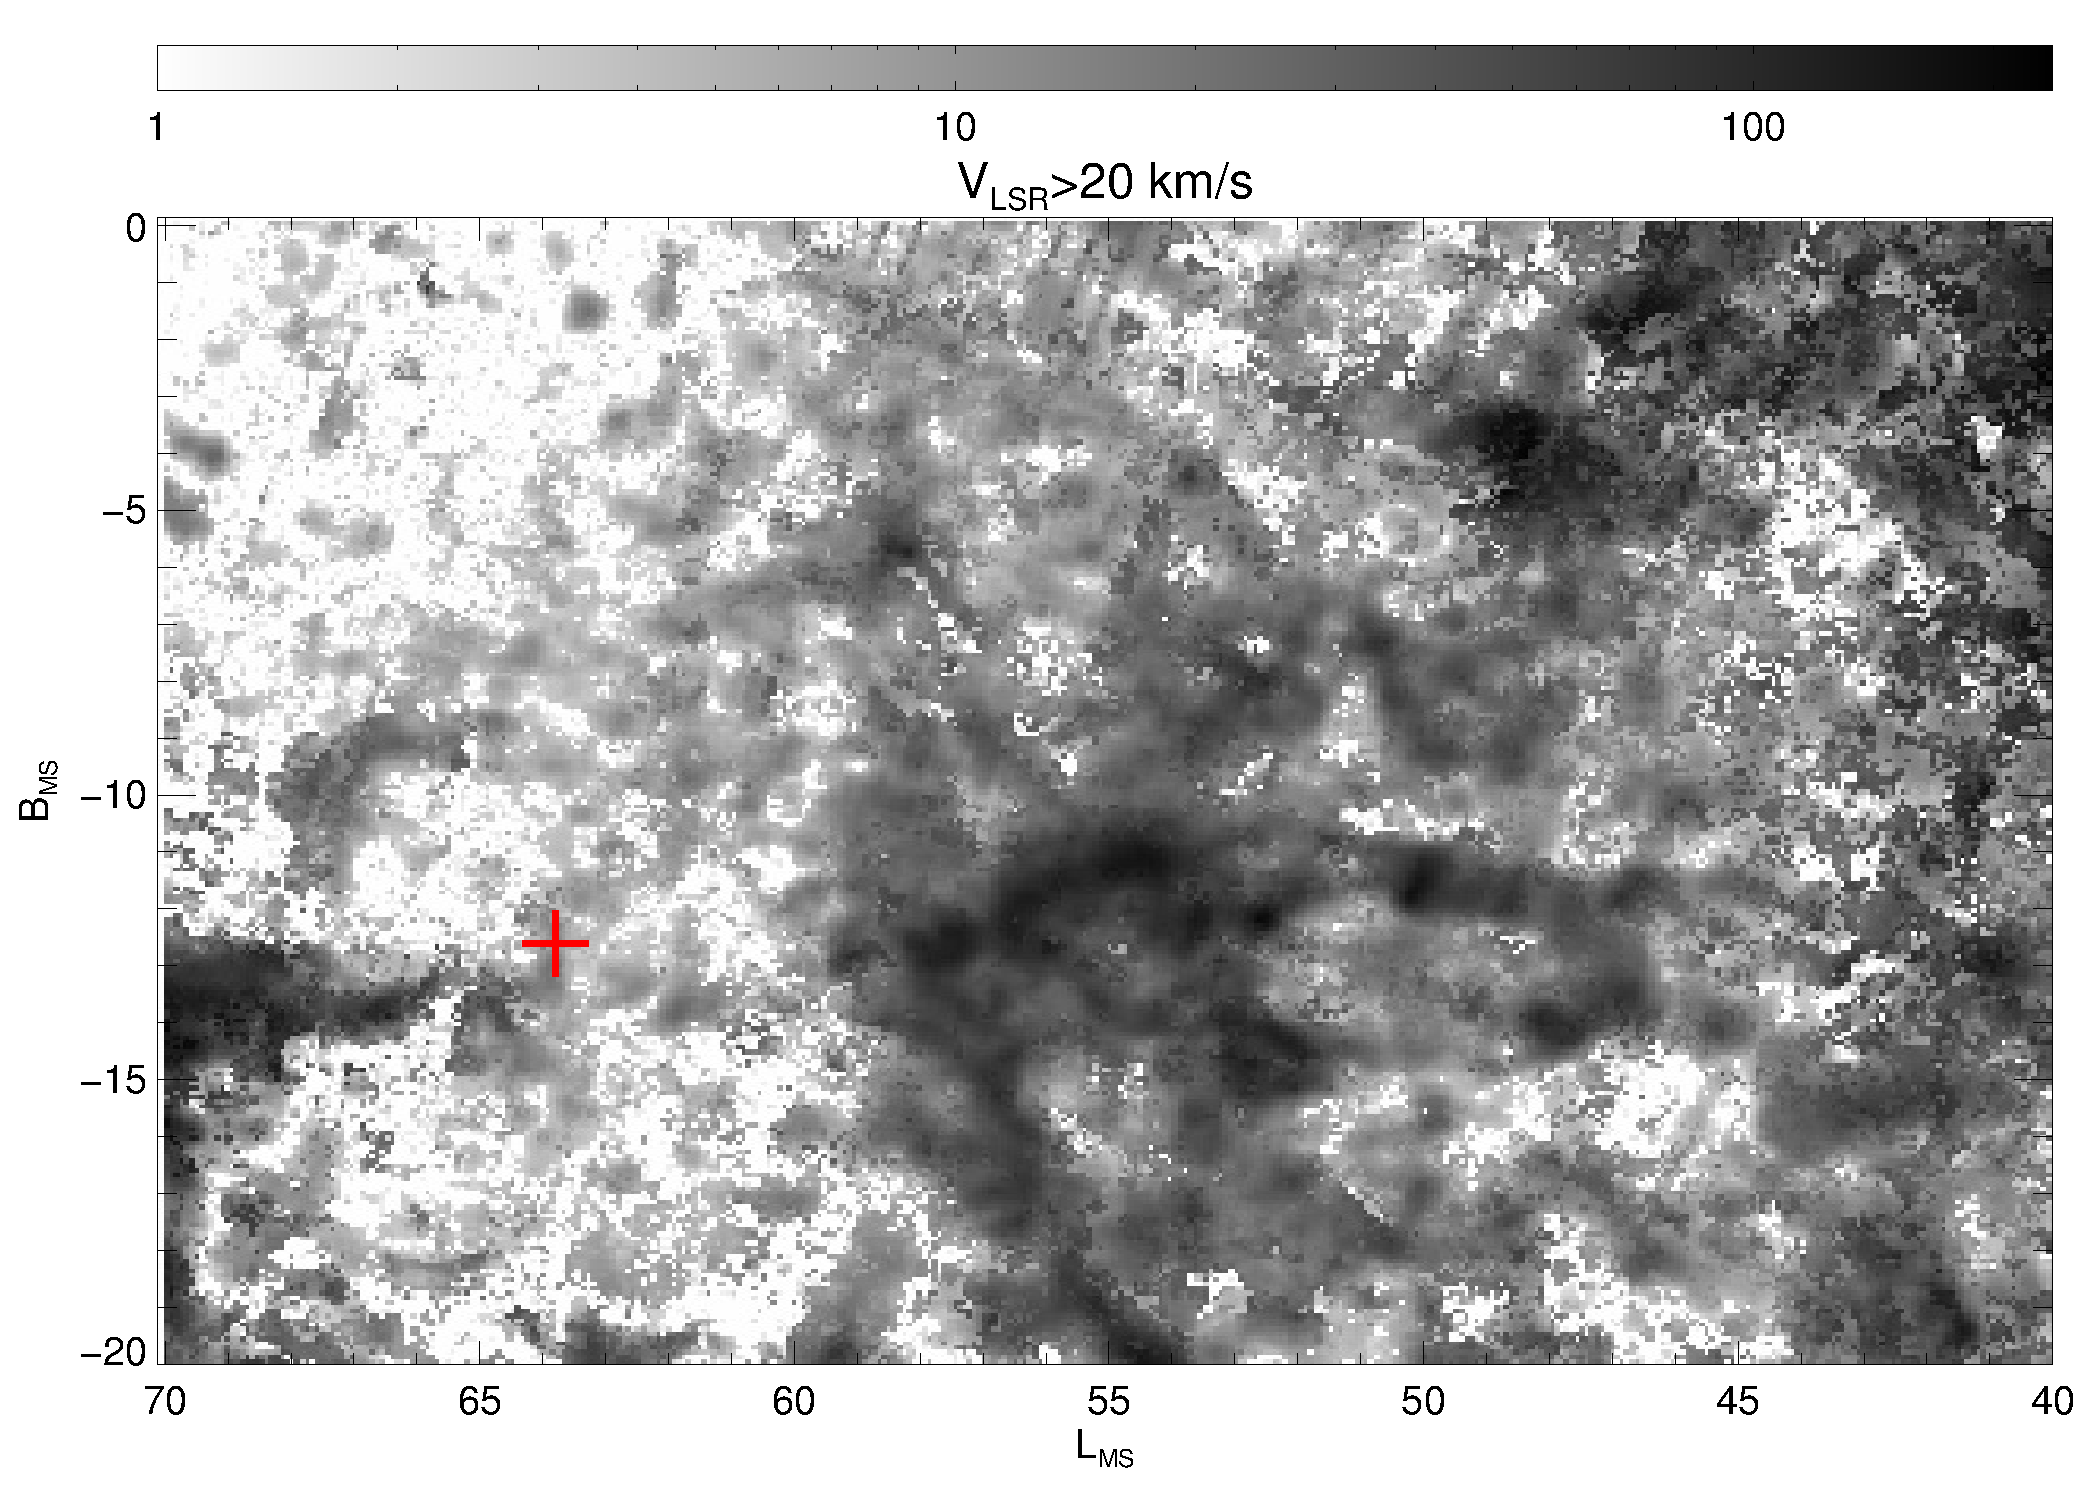
\includegraphics[width=8cm]{gass_mlatmlon.pdf}
\caption{GASS \hi column density in the region of LA II. The red cross marks the position
of the young cluster.}
\label{fig_gass}
\end{figure}

\begin{figure}
\centering
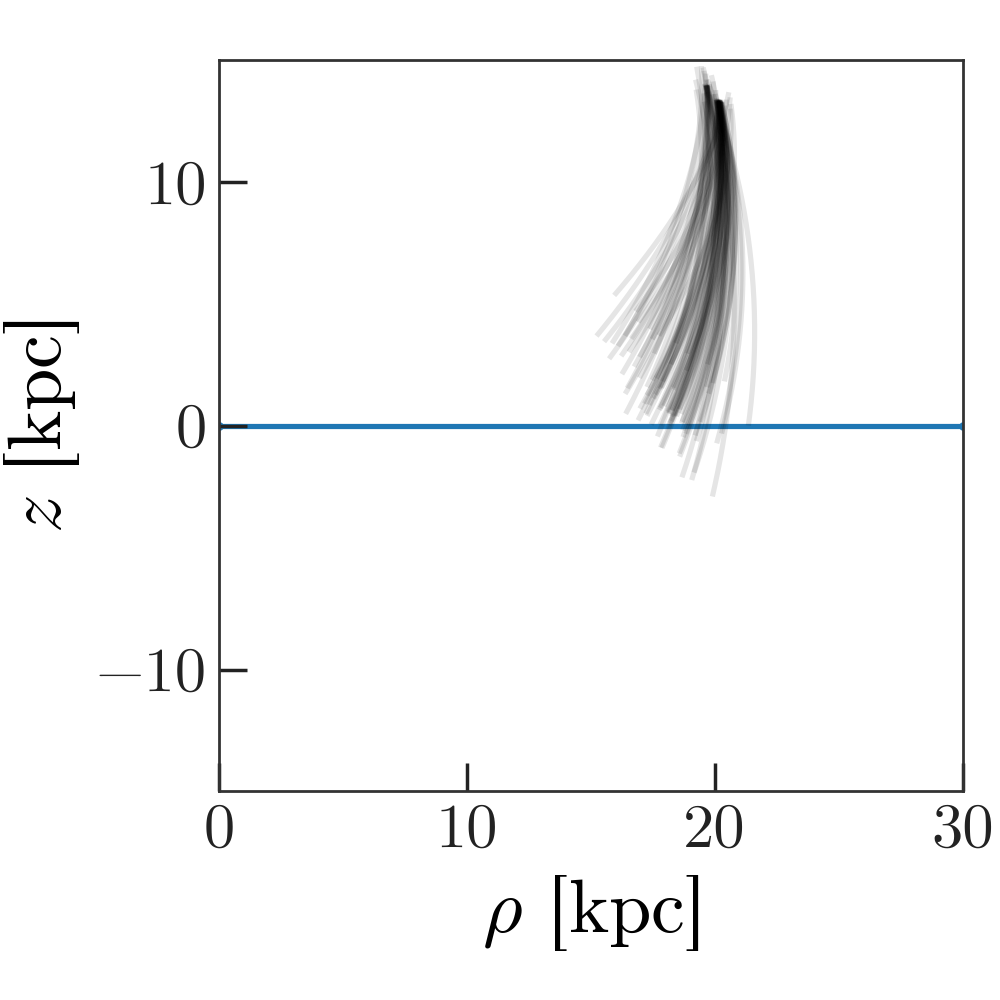
\includegraphics[width=8cm]{orbits.png}
\caption{Integrated orbits (over 60 Myr) of the star cluster using the Gaia DR2 proper motions, the
\hi~velocity and a distance of 25 kpc.  The orbits intersect the MW midplane about
60 Myr ago which is close to the age of the cluster.}
\label{fig_gass}
\end{figure}

\section{Discussion} \label{sec:discussion}

- Streams or clusters in the halo from star-formation from Sgr or dwarf gas

- Sgr young globular clusters: same thing as this? Indication of when Sgr lost its gas?

- Stars have the right metallicity to be SMC gas, I think

- TODO: where would interaction point between LMC gas and MW disk gas be today? ~150–200 Myr ago is almost 1 complete disk rotation. see Bekki:2008


\section{Conclusion} \label{sec:conclusion}

We have identified a young, metal-poor stellar association in the Galactic halo --- named \clustername --- with an age $\tau \approx 150~\textrm{Myr}$, heliocentric distance $D \approx 30~\kpc$, and metallicity $\feh \approx -1.1$.
At its present day sky position, and at large distances, all significant quantities of \hi are associated with the leading arm of the Magellanic gas stream and thus it plausibly formed from Magellanic stream gas.
The age of the cluster is broadly consistent with the time it would have crossed the Galactic midplane, suggesting the possibility that interaction with the Milky Way disk or tidal compression could have triggered this star formation event.
The discovery of \clustername\ provides a critical distance constraint to the Magellanic stream and will aid future Magellanic system and Milky Way modeling efforts.
It also provides an opportunity to study star formation in a unique environment, unlike that of the Milky Way disk or any other cluster-forming region.
The serendipitous discovery of this cluster is a reminder that the combined value of the \gaia\ data with deep, large-area imaging surveys will provide many more [...].


\acknowledgments

It is a pleasure to thank
Lauren Anderson (Flatiron),
Ana Bonaca (Harvard),
Elena D'Onghia (UW Madison),
Dan Foreman-Mackey (Flatiron),
Raja Guhathakurta (UCSC),
Cliff Johnson (Northwestern),
Ekta Patel (Arizona),
Josh Peek (STScI),
Anil Seth (\todo{where?}),
and Erik Tollerud (STScI)
for useful suggestions and discussion.

This work has made use of data from the European Space Agency (ESA)
mission {\it Gaia} (\url{https://www.cosmos.esa.int/gaia}), processed by
the {\it Gaia} Data Processing and Analysis Consortium (DPAC,
\url{https://www.cosmos.esa.int/web/gaia/dpac/consortium}). Funding
for the DPAC has been provided by national institutions, in particular
the institutions participating in the {\it Gaia} Multilateral Agreement.

\todo{Dylan Simon, Nick Carreiro and SCC at Flatiron}

\todo{Flatiron Institute}

\appendix

\section{Queries}
\label{sec:queries}

Initial query to select very blue stars away from the Galactic plane:
\begin{verbatim}
SELECT * FROM gaiadr2.gaia_source
WHERE parallax < 1
AND (bp_rp > -0.5) AND (bp_rp < 0)
AND phot_g_mean_mag < 20
AND ABS(b) > 20
\end{verbatim}

Query to retrieve \gaia\ data around the blue, comoving group found and discussed in \sectionname~\ref{sec:data}:
\begin{verbatim}
SELECT *
FROM gaiadr2.gaia_source
WHERE (parallax < 1 OR parallax IS NULL)
    AND ra > 173.5 AND ra < 185.5
    AND dec > -35.0 AND dec < -23.0
\end{verbatim}

\software{
    \package{Astropy} \citep{astropy, astropy:2018},
    \package{dustmaps}\footnote{\url{https://github.com/gregreen/dustmaps}},
    \package{emcee} \citep{emcee},
    \package{gala} \citep{gala},
    \package{IPython} \citep{ipython},
    \package{matplotlib} \citep{mpl},
    \package{numpy} \citep{numpy},
    \package{schwimmbad} \citep{schwimmbad},
    \package{scipy} \citep{scipy}
}

\bibliographystyle{aasjournal}
\bibliography{ms}

\end{document}
